\section*{Übung 7}
\subsection*{Aufgabe 1}
\subsubsection*{Lösungsidee}
Es werden Operationen zur Zeichenkettenverwaltung erstellt. Reversed liefert mithilfe einer For Schleife einen umgekehrten String zurück. StripBlanks arbeitet mit Call By Reference, und setzt den übergebenen String auf einen neuen String in dem nur Zeichen eingefügt wurden die keine Leerzeichen sind. 
ReplaceAll arbeitet mit subString und einem result String. An den result String wird ein subString angefügt, der die Zeichen von Position 1 im orignal String bis zur ersten Position der vorkommenden Zeichenkette -1 (weil sonst das erste Zeichen der Zeichenkette mit kopiert wird), enthält. Danach wird das zu ersetzende Wort angefügt und ein neuer subString erstellt der alle Zeichen, nach der Position + der Länge des alten Wortes, vom Original String enthält. Darauf wird wieder überprüft ob der zu ersetzende String im subString enthalten ist.
\newline

\lstinputlisting[language=Pascal] {../StringOperations.pas}
\begin{figure}[H]
	\centering
	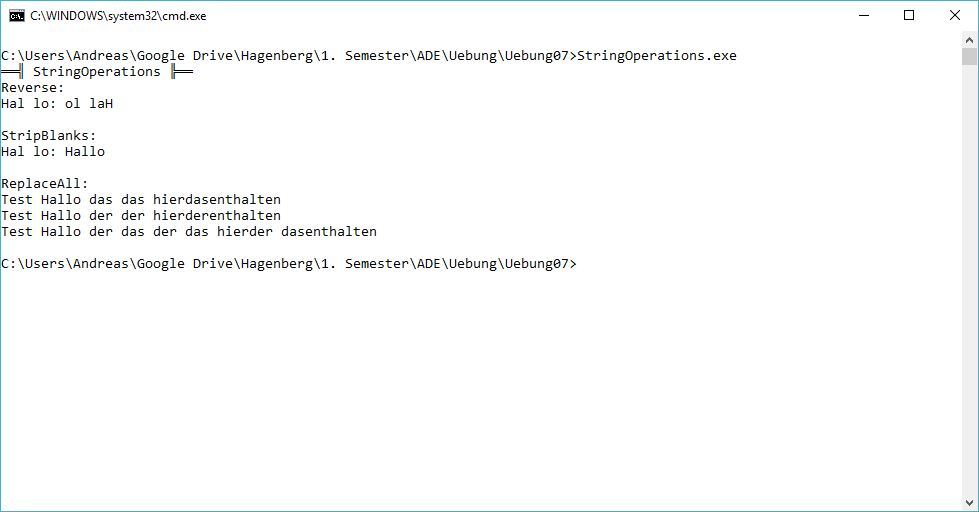
\includegraphics[scale=0.6]{./pictures/StringOperations.png}
	\caption{Testfälle Reverse, StripBlanks, ReplaceAll}
	\label{fig: String Operationen}
\end{figure}

\section*{Testfälle}
Bei Reverse wird der umgekehrte String ausgegeben.
StripBlanks zeigt das Leerzeichen aus einem String entfernt werden.
Bei ReplaceAll wird zuerst ein String durch einen komplett anderen ersetzt.
Die zweite Ausgabe zeigt das das ersetzen auch funktioniert wenn der neue String gleich ist mit dem alten oder der alte String in dem neuen enthalten ist.

\newpage

\subsection*{Aufgabe 2}
\subsubsection*{Lösungsidee}
Die Plausibilitätsüberprüfung von Messwerten kann auf verschiedene Arten gelöst werden.
Die drei hier verwendeten Arten:
\begin{itemize}
\item Globale Variablen
\item Lokale Variablen
\item Unit
\end{itemize}
Bei Globalen Variablen ist der große Nachteil/Vorteil das sie überall im Programm verwendet werden können. Bei Lokalen Variablen ist der Nachteil das sie nur innerhalb des Hauptprogrammes verwendet werden können. Die Unit verwendet ihre eigenen Variablen und greift auch selbst auf diese zu. Damit kann ohne Variablen Initialisierung im Hauptprogramm trotzdem ein Messwert überprüft werden. Alle drei Arten "merken" sich die vorherige Zeit und Temperatur und überprüfen damit ob die Temperatur plausibel ist. Zusätzlich müssen bei allen drei Arten die Werte mindestens einmal initialisiert werden sonst funktioniert die Überprüfung nicht.
\newline

\lstinputlisting[language=Pascal] {../isPlausible_PseudoCode.pas}
\lstinputlisting[language=Pascal] {../temp.pas}
\begin{figure}[H]
	\centering
	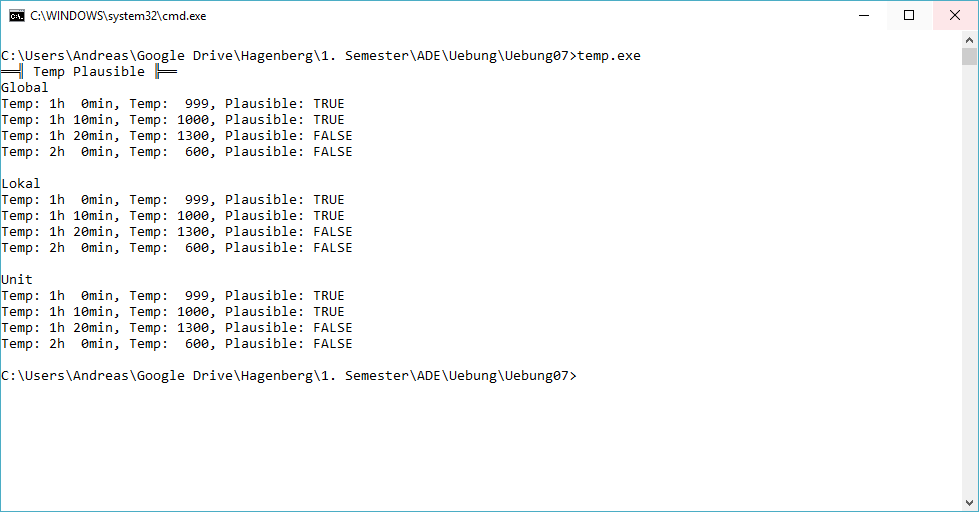
\includegraphics[scale=0.6]{./pictures/temp.png}
	\caption{Testfälle Temperatur Messung}
	\label{fig: Temp Messung}
\end{figure}

\section*{Testfälle}
Die Testfälle zeigen die Messwertüberprüfung bei allen drei Arten.
\newpage

\subsection*{Aufgabe 3}
\subsubsection*{Lösungsidee Übung 2}
Bei der Quadratwurzelberechnung soll mithilfe einer Reellen Zahl und einer Fehlerschranke die Quadratische Wurzel der Reellen Zahl berechnet werden. Dazu muss die Richtigkeit der Eingabe überprüft werden und entsprechende Fehlermeldungen ausgegeben werden. Nach der Überprüfung der Eingabe soll mithilfe der Newtonsche Iterationsformel eine Näherung für $y \approx \sqrt{x}$ berechnet werden. Mithilfe der Formel $ y1 = \frac{1}{2}(y0 + \frac{x}{y_{0}})$ und einer Repeat Until Schleife die nach 50 Iterationen abbricht wird eine Näherung für die Eingabe berechnet.
\newline
\lstinputlisting[language=Pascal] {../quadratwurzel_old.pas}

\newpage
\subsubsection*{Anmerkungen}
Für die Lösungsidee ist nicht notwendig wie diese Formel aussieht solange sie im Programm verwendet wird. Der Programmstil selbst zeichnet sich durch einen nicht eingehaltenen Standard aus, wie etwa das klein schreiben der Schlüsselwörter. Die Näherung selbst kann in eine eigene Funktion ausgelagert werden, damit kann die Funktion überall einfach verwendet werden, falls Änderungen an der Näherung gemacht werden muss somit nicht überall der Programm Code verändert werden. Die Repeat Until Schleife kann durch eine While Schleife ersetzt werden.
\newline

\subsubsection*{Lösungsidee Neu}
Mithilfe einer Prozedur und Call By Reference wird mit einer Näherungsformel die Quadratwurzel einer Zahl ausgerechnet. Wenn nach 50 Iterationen keine Konvergenz gefunden wurde wird abgebrochen. Zusätzlich werden die Eingaben auf Fehler überprüft und entsprechende Fehlermeldungen ausgegeben.
\newline
\lstinputlisting[language=Pascal] {../quadratwurzel_new.pas}
\begin{figure}[H]
	\centering
	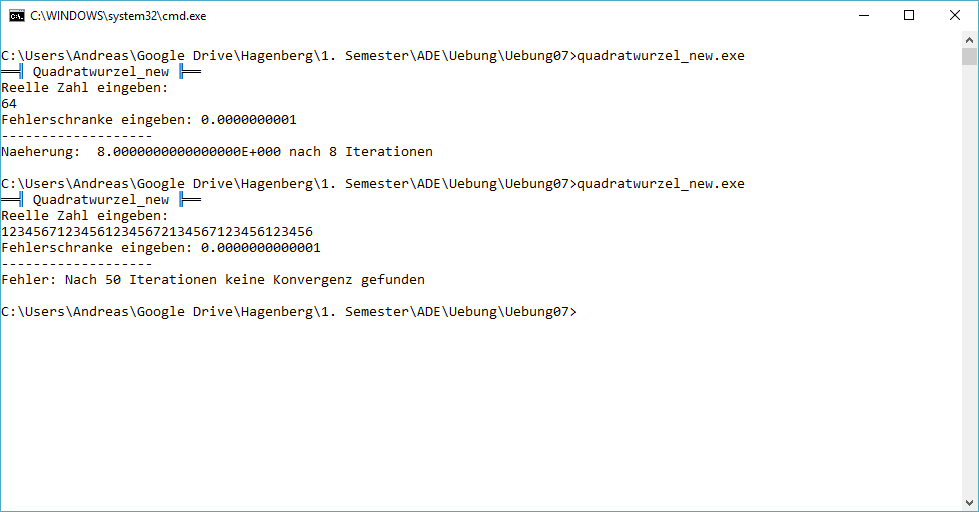
\includegraphics[scale=0.6]{./pictures/quadratwurzel_new.png}
	\caption{Testfälle Quadratwurzel}
	\label{fig: Quadratwurzel Neu}
\end{figure}

\section*{Testfälle}
Die Testfälle zeigen die Ausgabe mit der überarbeiteten Version von Quadratwurzel.

\newpage

